\subsection{Valg av modellorden, og validering}
I forrige delkapittel lovpriste vi PCA-ens evne til å reduserte dimensjonen til en datamatrise uten at vi mister informasjon. Men hvor mye kan man egentlig redusere denne dimensjonen, og hvordan velger man hvilken informasjon man har råd til å kaste vekk? Det er denne typen problemstilling \textbf{modellordenseleksjon} handler om.

\subsubsection{Problemformulering}
Modellordenseleksjon er et problem i mengden av \textbf{modellseleksjonsproblemer}. Disse går ut på å velge en statistisk modell av flere gitt et datasett som skal forklares. Dette kan virke enkelt (bare velg modellen som gir lavest kvadratavvik for datasettet da vel!), men få datasett representerer virkeligheten 100\%. Bias vs. varians-tradeoffen gjør seg dessverre gjeldende og tvinger oss til å balansere på en knivsegg mellom over- og undertilpassing av modellen vår. Uff.

\subsubsection{Motivasjon}
Anta at vi har et datasett med én observasjon, $y \sim \mathcal{N}(\mu, \sigma^2)$, som estimeres vha. funksjonen $\hat{\mu} (y)$. Hvordan vet vi hvor god denne stimatoren er? Vi kan jo forsøke å finne MSE av estimatoren direkte, det er bare ett problem (her har jeg vært litt lat med å vise utregninger):

\begin{equation}
\mathbb{E} [(\mu - \hat{\mu})^2] = \cdots = -n \sigma^2 + \mathbb{E} [(y - \mu)^2] + \underbrace{2 \textrm{cov}(y, \mu)}_{\textrm{trøbbel}}
\end{equation}

Det siste leddet har man vanligvis ikke kjennskap til. Hvordan kan vi da anslå hvor god en estimator er, når man ikke er så heldig å ha fått utdelt et testsett å teste på?

\subsubsection{Kryssvalidering}
Om man ikke har et dedikert testsett å validere en modell på, kan man lage sitt eget ved å dele opp treningssettet. Dette kalles \textbf{kryssvalidering}. Ulike måter å dele opp på gir ulike former for kryssvalidering.

Det er ønskelig å ha et så stort treningssett som mulig, så et naturlig valg vil være å kun utelate én observasjon som treningssett. Ved å utelate en og en observasjon, kan man regne ut $n$ ulike MSE-er. Gjennomsnittet av disse gir \textbf{Leave One Out Cross-Validation (LOOCV)}.

Å tilpasse en modell $n$ ganger for et datasett på $n$ observasjoner kan være beregningskrevende (i tillegg til å gi høy varians i MSE, uten at jeg helt kan forklare hvorfor). I stedet for å utelate én observasjon som treningssett $n$ ganger, kan man utelate $\frac{n}{k}$ observasjoner $k$ ganger, og regne ut gjennomsnittet av de $k$ MSE-ene dette resulterer i. Dette kalles \textbf{k-Fold Cross-Validation}, og regnes altså ut som

\begin{equation}
	\textrm{CV}_{(k)} = \frac{1}{k} \sum_{i=1}^{k} \textrm{MSE}_i
\end{equation}

Om man vil ha en likning for LOOCV får man det ved å sette $k = n$ her.

Uansett hvordan man velger $k$, er det viktig å sørge for at naturlige strukturer ikke brytes. For eksempel burde et datasett av vær over flere år deles opp i år, slik at sesongvariasjoner plukkes opp. Fullstendig tilfeldig inndeling vil her kunne gi merkelige resultater.

\subsubsection{Valg av antall PCA-komponenter}
Et spesialtilfelle av modellordenseleksjon er valg av antall PCA-komponenter å beholde. Noen muligheter som nevnes er
\begin{itemize}
	\item Bartletts test
	\item ``Broken stick''-testesn
	\item Behold alle egenverdier $\leq 1$ (for variabler skalert til å ha enhetsvarians)
	\item La summen av PC-ene forklare 95\% av variansen (ikke anbefalt)
	\item Bruk et SCREE-plot til å tolke viktigheten av komponentene
\end{itemize}
I kombinasjon med sistnevnte kan kjennskap til systemet og dens dimensjonalitet være nyttig å bruke. Dette gjelder også når man skal gjøre kryssvalidring av PCA-modeller. I tillegg er det viktig å sjekke stabiliteten (dvs. sensitivitet til variasjoner i treninsdata). Om dette er uklart burde følgende figur forklare alt

\begin{figure}[h]
	\centering
	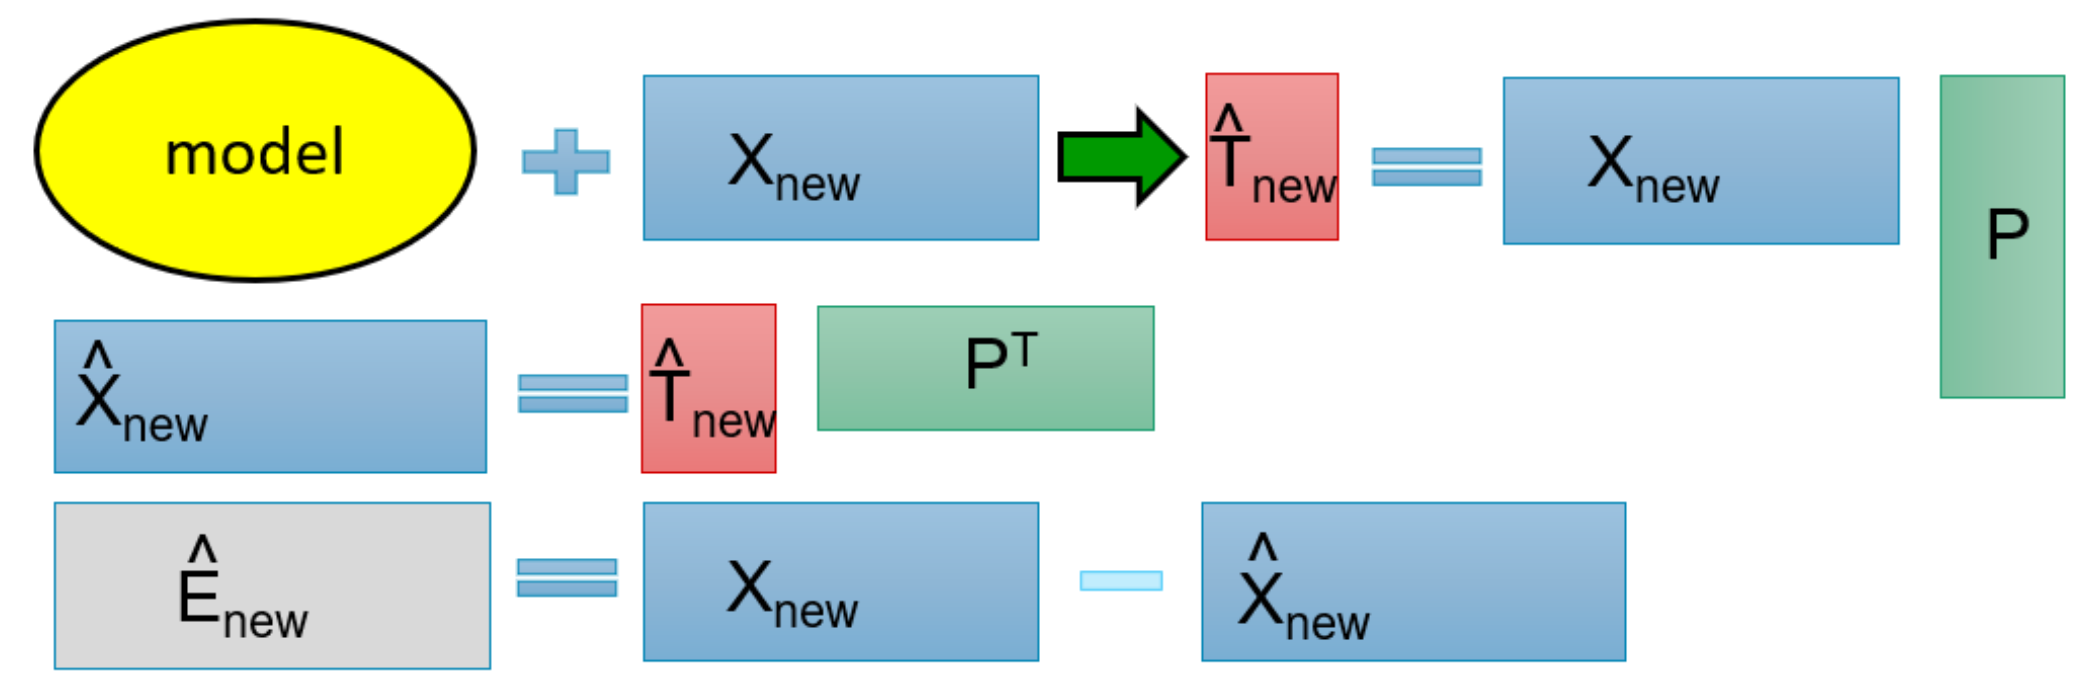
\includegraphics[width=\textwidth]{figurer/pca_kryssvalidering}
	\caption{Selvforklarende figur}
	\label{fig:pca_kryssvalidering}
\end{figure}

\subsubsection{Informasjonskriterier}
Om man har begrenset med regnekapasitet eller små datasett med dårlige muligheter for oppdeling, kan kryssvalidering være upraktisk å gjennomføre. Da kan at alternativ være å bruke et \textbf{informasjonskriterie}. Disse gir oss estimatorer for MSE som kompenserer for det faktum at MSE på treningssett typisk er underestimater.

Anta at vi for en modell av orden $n$, basert på et datasett $\mathcal(D)$, har gitt et estimat $\theta_n$. Observasjonen estimatet vårt er basert på er fordelt med sannsynlighetstettheten $p_n(\mathcal{D}, \theta_n)$. Vi ønsker å minimere avstanden (hva nå enn det måtte bety) til den faktiske fordelingen $p_0(\mathcal{D}, \theta_0)$. En naturlig måte å måle denne avstanden på er ved å bruke Kullback-Leibler-divergens, som måler informasjon tapt når man representerer $p_0$ ved $p_n$. Denne er gitt av

\begin{equation}
	K L\left(p_{0}, p_{n}\right):=\int \log \left(\frac{p_{0}\left({\mathcal{D}}, \theta_{0}\right)}{p_{n}\left({\mathcal{D}}, \theta_{n}\right)}\right) p_{0}\left({\mathcal{D}}, \theta_{0}\right) d {\mathcal{D}}
\end{equation}

Det kan vises at denne er lik $\mathbb{E}_{p_0} [\ell (\mathcal{D}, \theta_n)] + \textrm{ et eller annet uavhengig av } \theta_n$. Det siste leddet betyr at vi mister informasjon om absolutt informasjonstap, men om vi kun er interessert i å sammenligne ulike $\theta_n$ er ikke dette noe problem. Om vi finner et estimat av denne forventingsverdien kan vi minimere mhp. $n$, og dermed bestemme hvilken modell som er best etter dette kriteriet.

Akaike gjorde noen antagelser, fant et estimat, og fikk kriteriet dette resulterte i oppkalt etter seg (\textbf{AIC}). Dette er gitt av (der $\varepsilon$ er feil, typisk $y - \hat{y}$ e.l.)

\begin{equation}
	\textrm{AIC} = \frac{1}{N} \sum_{t = 1}^N \ell (\varepsilon (t, \theta_n)) + \frac{1}{N} \textrm{dim}(\theta_n)
\end{equation}

Under andre antakelser kan man finne andre kriterier. Et annet mye brukt kriterie (gjerne på mindre datasett, siden den ikke er en konsistent estimator) er det Bayesiske informasjonskriteriet (\textbf{BIC})

\begin{equation}
	\textrm{BIC} = \frac{1}{N} \sum_{t = 1}^N \ell (\varepsilon (t, \theta_n)) + \frac{\log N}{2N} \textrm{dim}(\theta_n)
\end{equation}

\subsubsection{Jackknifing og bootstrapping}


